%!TEX program = xelatex
\let\stop\empty

\documentclass[12pt,a4paper]{exam-zh}

%region 导言区
\usepackage{xeCJK}
\setCJKmainfont{Noto Serif CJK SC}
\usepackage{geometry}
\usepackage{array}
\usepackage{tikz}
\usepackage{amsmath}
\usepackage{wrapfig}
\usepackage{adjustbox}
\usepackage{enumitem}
\usepackage{fancyhdr}
\usetikzlibrary{quotes,angles}
\usepackage{scalerel}
\def\mcirc{\mathbin{\scalerel*{\circ}{j}}}
\def\msquare{\mathord{\scalerel*{\Box}{gX}}}

\usepackage{setspace}
\usepackage{eso-pic}
\usetikzlibrary{calc}
\newcommand{\ulinefill}[1]{\underline{\hspace{#1}}}
% \renewcommand{\choiceshook}{%
%     \setlength{\leftmargin}{18pt}%
% }
\geometry{margin=0cm,top=0.5cm,bottom=0.5cm}
%endregion



%region exam setup
\examsetup{
    % problem/label = \arabic*., 
    % 设置大题题号格式 
        question = {
        top-sep = 1em,      % 题头上方的间距（默认 0.25em）
        bottom-sep = 1em,   % 题号下方的间距（默认 0pt）
    },
    % 隐藏大题后的分值显示 
    problem/show-points = false,
    % 调整小题列表的缩进和间距
    list/step-name = {}, 
    solution = {
    show-solution = show-move, % 答案自动移动到卷末
    label-content = {answer},  % 答案区的标题文字
    show-qed = true            % 在解答末尾显示结束符号 ◻ 
  },
    page = {
    size = a4paper,           % 设定纸张大小 
    foot-content = { - ; - }  % 页脚显示为 -1-, -2- 格式 
  }
}
\setlist[enumerate,1]{
    label=(\alpha*), 
    itemsep=0.5em, 
    leftmargin=2em, 
    after=\hfill % 配合您之前要求的百分比靠右样式
}
%endregion

%region 卷面变量设置
% ==========================
% 卷面变量设置（只需改这里）
% ==========================
\newcommand{\papercode}{SC 06}
\newcommand{\examtitle}{2026年金宝培元独立中学半年考}
\newcommand{\examlevel}{高中组}
\newcommand{\examsubject}{高级数学(I)}
\newcommand{\sidebartext}{高级数学(I)/一}
\newcommand{\papername}{试卷二}
\newcommand{\papertype}{作答题}
\newcommand{\examdate}{2026年5月21日}
\newcommand{\examtime}{9.00 a.m.－11.00 a.m.}
\newcommand{\examduration}{2 小时}
\newcommand{\questionpages}{四面}
\newcommand{\paperonepercentage}{40\%}
\newcommand{\papertwopercentage}{60\%}
\newcommand{\requiredgroupnotice}{甲组：必答题（20\%）（5 题全答）}
\newcommand{\electivegroupnotice}{乙组：选答题（40\%）（7 题选答 4 题）}
\newcommand{\requiredgrouptitle}{甲组：必答题（5 题全答）}
\newcommand{\electivegrouptitle}{乙组：选答题（7 题选答 4 题）}
\newcommand{\setterteacher}{蔡杰庆师}
\newcommand{\reviewteacher}{杨丽芳师}
\newcommand{\auditteacher}{雷泳健师}
%endregion

\begin{document}


%region 封面
\AddToShipoutPictureFG*{%
  \put(31,104){\color{black}\rule{16pt}{66pt}}%
  \put(37,112){\makebox(0,0)[lb]{\rotatebox{90}{\color{white}\bfseries\footnotesize \sidebartext}}}%
  \put(24,18){\makebox(0,0)[lb]{\small 版权所有}}%
  \put(520,18){\makebox(0,0)[lb]{\bfseries\small 【机密】}}%
}

\begin{center}
  {\zihao{3}\bfseries \examtitle\par}
  \vspace{1.0em}
  {\zihao{4}\bfseries \examlevel\par}
  \vspace{1.0em}
  {\zihao{2}\bfseries \examsubject\par}
  \vspace{0.2em}
  {\small (\papercode)\par}
\end{center}

\vspace{1.3em}

\begin{center}
  \begin{tabular}{c}
    \papername\hspace{2em}\papertype\\[-0.1em]
    \noalign{\hrule height 0.4pt}
    日期：\examdate\\[-0.05em]
    时间：\examtime\\[-0.05em]
    （\examduration）\\
    \noalign{\hrule height 0.4pt}
  \end{tabular}
\end{center}

\vspace{1.0em}

{\zihao{4}\bfseries 考 生 须 知\par}
\vspace{0.55em}

\begin{enumerate}[label=（\arabic*）,leftmargin=2.8em,itemsep=0.38em]
  \item 本科试卷共分两份：\\
  \hspace*{1.3em}试卷一：选择题（\paperonepercentage），\\
  \hspace*{1.3em}试卷二：作答题（\papertwopercentage）。
    
  \item
  试卷二分为两组：\\
  \hspace*{1.3em}\textbf{\requiredgroupnotice}\\
  \hspace*{1.3em}\textbf{\electivegroupnotice。}

  \item \textbf{每题必须用新的一张纸作答。}

  \item 只可用蓝色或黑色的原子笔书写，惟可用铅笔画图。

  \item 不必抄题，惟试题号码必须书写清楚。

  \item 所有演算必须清楚地写出。必要的几何图形必须画出。

  \item 可使用所规定的电子计算机进行演算，除非题目限制。

  \item 答卷必须依试题号码次序排列，并且将\textbf{积分表}（电脑卡）置于上\\
  面，合订成一本。

  \item 试卷二作答题共印\questionpages，最后一面空白。
\end{enumerate}

\vspace{1.0em}

\begin{center}
  \fbox{\rule{0pt}{1.15em}\hspace{1.2em}{\bfseries 未经正式宣布\quad 不得翻看内页}\hspace{1.2em}}
\end{center}

\vspace{1.2em}

\noindent
（考生姓名：\ulinefill{4.4cm}\hfill 考生编号：\ulinefill{4.3cm}）
%endregion


\newpage


% ============================================================
%  试卷二：作答题（甲组必答题 + 乙组选答题）
%  格式：\begin{question}...\end{question}
%        \begin{solution}...\end{solution}
% ============================================================

%region 甲组：必答题

{\zihao{4}\bfseries \requiredgrouptitle\par}
\vspace{0.8em}

%region 甲组 第 1 题
\begin{question}
    已知函数 $f(x) = a + \dfrac{b}{x+5}$ 且 $f(-4) = -1$，$f(-1) = 2$。
    \begin{enumerate}[label=(\alph*)]
        \item 求 $a$ 及 $b$ 的值。\hfill(2\%)
        \item 求 $f^{-1}(x)$。\hfill(2\%)
    \end{enumerate}
\end{question}

\begin{solution}
    \textbf{(a) 求 $a$ 及 $b$：} \\
    将 $f(-4) = -1$ 代入：
    \[
        a + \frac{b}{-4+5} = -1 \implies a + b = -1. \quad \cdots (1)
    \]
    将 $f(-1) = 2$ 代入：
    \[
        a + \frac{b}{-1+5} = 2 \implies a + \frac{b}{4} = 2. \quad \cdots (2)
    \]
    $(1) - (2)$：$b - \dfrac{b}{4} = -3 \implies \dfrac{3b}{4} = -3 \implies b = -4$。 \\
    代回 $(1)$：$a + (-4) = -1 \implies a = 3$。 \\
    故 $a = 3$，$b = -4$。

    \textbf{(b) 求 $f^{-1}(x)$：} \\
    令 $y = 3 + \dfrac{-4}{x+5}$，解 $x$：
    \[
        y - 3 = \frac{-4}{x+5} \implies x + 5 = \frac{-4}{y-3} \implies x = \frac{-4}{y-3} - 5.
    \]
    故 $f^{-1}(x) = \dfrac{-4}{x-3} - 5 = \dfrac{-4 - 5(x-3)}{x-3} = \dfrac{11-5x}{x-3}$，其中 $x \ne 3$。
\end{solution}
%endregion

%region 甲组 第 2 题
\begin{question}[points = 4]
    如图所示为一长方体，其中 $AB = 8\text{ cm}$，$BC = 6\text{ cm}$，$CG = 4\text{ cm}$。求 $AG$ 与平面 $CDHG$ 所成的角。

    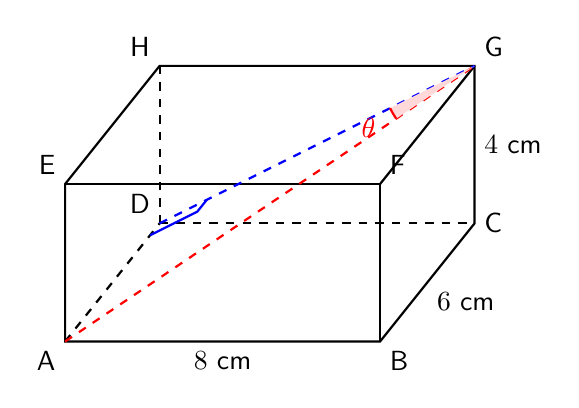
\begin{tikzpicture}[
    % 设置 3D 透视视角的 x, y, z 轴投影向量
    x={(-0.4cm,-0.5cm)},
    y={(1cm,0cm)},
    z={(0cm,1cm)},
    scale=0.5,
    font=\sffamily
]
    % 1. 定义长方体各顶点坐标 (基于 D 为原点)
    \coordinate (D) at (0,0,0);
    \coordinate (C) at (0,8,0);
    \coordinate (H) at (0,0,4);
    \coordinate (G) at (0,8,4);
    \coordinate (A) at (6,0,0);
    \coordinate (B) at (6,8,0);
    \coordinate (E) at (6,0,4);
    \coordinate (F) at (6,8,4);

    % 2. 绘制被遮挡的边（虚线）
    \draw[dashed, thick] (A) -- (D);
    \draw[dashed, thick] (D) -- (C);
    \draw[dashed, thick] (D) -- (H);

    % 3. 绘制可见的边（实线）
    \draw[thick] (A) -- (B) -- (C) -- (G) -- (H) -- (E) -- cycle;
    \draw[thick] (B) -- (F) -- (E);
    \draw[thick] (F) -- (G);

    % 4. 绘制求解角度的辅助线（AG 和投影线 DG）
    \draw[dashed, thick, blue] (D) -- (G);
    \draw[dashed, thick, red] (A) -- (G);

    % 5. 标注顶点字母
    \node[below left] at (A) {A};
    \node[below right] at (B) {B};
    \node[right] at (C) {C};
    \node[above left] at (D) {D};
    \node[above left] at (E) {E};
    \node[above right] at (F) {F};
    \node[above right] at (G) {G};
    \node[above left] at (H) {H};

    % 6. 标注题目给定的边长
    \node[below] at ($(A)!0.5!(B)$) {$8$ cm};
    \node[below right] at ($(B)!0.5!(C)$) {$6$ cm};
    \node[right] at ($(C)!0.5!(G)$) {$4$ cm};

    % 7. 标注底面的空间直角符号 \angle ADG
    \coordinate (D1) at ($(D)!0.1!(A)$);
    \coordinate (D2) at ($(D)!0.15!(G)$);
    \coordinate (D3) at ($(D1)+(D2)-(D)$);
    \draw[thick, blue] (D1) -- (D3) -- (D2);

    % 8. 标注目标角 \angle AGD (用红色扇形表示)
    \pic [draw, thick, red, fill=red!15, angle radius=1.2cm, "$\theta$", angle eccentricity=1.3] {angle = D--G--A};

\end{tikzpicture}
 \hfill (4\%)
\end{question}

\begin{solution}
    \textbf{解析：} \\
    要求直线 $AG$ 与平面 $CDHG$ 所成的角，需要先找到直线 $AG$ 在该平面上的投影。 \\
    因为该几何体为长方体，所以棱 $AD$ 垂直于平面 $CDHG$，即 $AD \perp$ 平面 $CDHG$。 \\
    因此，点 $A$ 在平面 $CDHG$ 上的投影为点 $D$。 \\
    又因为点 $G$ 本身就在平面 $CDHG$ 上，所以直线 $AG$ 在平面 $CDHG$ 上的投影为直线 $DG$。 \\
    $\therefore$ 直线 $AG$ 与平面 $CDHG$ 所成的角即为 $\angle AGD$。 \\
    在 $\text{Rt}\triangle ADG$ 中，$\angle ADG = 90^\circ$。 \\
    已知 $AD = BC = 6\text{ cm}$。 \\
    在矩形 $CDHG$ 中，$CD = AB = 8\text{ cm}$，$DH = CG = 4\text{ cm}$，根据勾股定理可得 $DG$ 的长度：
    \[ \displaystyle DG = \sqrt{CD^2 + DH^2} = \sqrt{8^2 + 4^2} = \sqrt{64 + 16} = \sqrt{80} = 4\sqrt{5}\text{ cm} \]
    在 $\text{Rt}\triangle ADG$ 中，利用正切函数求 $\angle AGD$：
    \[ \displaystyle \tan \angle AGD = \frac{AD}{DG} = \frac{6}{4\sqrt{5}} = \frac{3}{2\sqrt{5}} = \frac{3\sqrt{5}}{10} \]
    （注：也可求得空间对角线 $\displaystyle AG = \sqrt{8^2 + 6^2 + 4^2} = 2\sqrt{29}$，得 $\displaystyle \sin \angle AGD = \frac{6}{2\sqrt{29}} = \frac{3\sqrt{29}}{29}$） \\
    $\therefore AG$ 与平面 $CDHG$ 所成的角为 $\displaystyle \arctan\left(\frac{3\sqrt{5}}{10}\right)$ （或 $\displaystyle \arcsin\left(\frac{3\sqrt{29}}{29}\right)$）。
\end{solution}
%endregion

%region 甲组 第 3 题
\begin{question}
    已知圆 $x^2 + y^2 - 4x + 2y - 4 = 0$ 与 $y$ 轴相交于 $A$、$B$ 两点。
    \begin{enumerate}[label=(\alph*)]
        \item 求圆心及半径。\hfill(2\%)
        \item 求 $AB$ 的长。\hfill(2\%)
    \end{enumerate}
\end{question}

\begin{solution}
    \textbf{(a) 配方求圆心及半径：} \\
    \[
        (x^2 - 4x + 4) + (y^2 + 2y + 1) = 4 + 4 + 1
        \implies (x-2)^2 + (y+1)^2 = 9.
    \]
    圆心为 $(2,\ -1)$，半径 $r = 3$。 \\

    \textbf{(b) 求 $AB$ 的长：} \\
    令 $x = 0$ 代入原方程：$0 + y^2 + 0 + 2y - 4 = 0 \implies y^2 + 2y - 4 = 0$。 \\
    由韦达定理，两根 $y_A + y_B = -2$，$y_A y_B = -4$。 \\
    \[
        AB = |y_A - y_B| = \sqrt{(y_A+y_B)^2 - 4y_Ay_B} = \sqrt{4 + 16} = \sqrt{20} = 2\sqrt{5}\ \text{cm}.
    \]
\end{solution}
%endregion

%region 甲组 第 4 题
\begin{question}
    七个小矮人的身高（cm）为：$121,\ 116,\ 112,\ 124,\ 127,\ 115,\ 118$。
    \begin{enumerate}[label=(\alph*)]
        \item 小红帽加入这群小矮人后，平均身高没有改变。求小红帽的身高。\hfill(2\%)
        \item 小木偶加入这群小矮人后，身高的中位数增加了 $1\ \text{cm}$。求小木偶的身高。\hfill(2\%)
    \end{enumerate}
\end{question}

\begin{solution}
    \textbf{(a) 求小红帽身高：} \\
    原七人身高总和：$121+116+112+124+127+115+118 = 833\ \text{cm}$。 \\
    原平均数：$\bar{x} = \dfrac{833}{7} = 119\ \text{cm}$。 \\
    小红帽加入后平均不变，即小红帽身高 $= 119\ \text{cm}$。 \\

    \textbf{(b) 求小木偶身高：} \\
    将七人身高排序：$112,\ 115,\ 116,\ 118,\ 121,\ 124,\ 127$。 \\
    原中位数（第 4 位）$= 118\ \text{cm}$。 \\
    小木偶加入后共 8 人，中位数为第 4、5 位平均，且中位数增加 $1\ \text{cm}$，即新中位数 $= 119\ \text{cm}$。 \\
    设小木偶身高为 $h$。加入后第 4、5 位平均须为 $119$：
    \[
        \frac{\text{第4位} + \text{第5位}}{2} = 119 \implies \text{第4位} + \text{第5位} = 238.
    \]
    原排序第4位为 $118$，第5位为 $121$，和为 $239 \ne 238$。 \\
    若 $h$ 插入第4、5位之间（$118 \le h \le 121$），新序列第4、5位为 $h$ 和 $121$（或 $118$ 和 $h$），需：
    \[
        \frac{118 + h}{2} = 119 \implies h = 120\ \text{cm}.
    \]
    故小木偶身高为 $120\ \text{cm}$（满足 $118 \le 120 \le 121$，验证正确）。
\end{solution}
%endregion

%region 甲组 第 5 题
\begin{question}[points = 4]
    求矩阵 $\displaystyle \begin{pmatrix} 3 & 5 \\ 4 & 6 \end{pmatrix}$ 的逆矩阵。据此，解方程组 $\displaystyle \begin{cases} 3x + 5y = 9 \\ 4x + 6y = 10 \end{cases}$。\hfill(4\%)
\end{question}

\begin{solution}
    \textbf{解析：} \\
    \textbf{第一步：求逆矩阵} \\
    设矩阵 $\displaystyle A = \begin{pmatrix} 3 & 5 \\ 4 & 6 \end{pmatrix}$。首先计算其行列式 $\displaystyle \det(A)$：
    \[ \displaystyle \det(A) = 3 \times 6 - 5 \times 4 = 18 - 20 = -2 \]
    利用二阶矩阵求逆公式 $\displaystyle \begin{pmatrix} a & b \\ c & d \end{pmatrix}^{-1} = \frac{1}{ad-bc} \begin{pmatrix} d & -b \\ -c & a \end{pmatrix}$，得：
    \[ \displaystyle A^{-1} = \frac{1}{-2} \begin{pmatrix} 6 & -5 \\ -4 & 3 \end{pmatrix} = \begin{pmatrix} -3 & \frac{5}{2} \\ 2 & -\frac{3}{2} \end{pmatrix} \]

    \textbf{第二步：利用逆矩阵解方程组} \\
    原方程组可以写成矩阵形式 $\displaystyle AX = B$：
    \[ \displaystyle \begin{pmatrix} 3 & 5 \\ 4 & 6 \end{pmatrix} \begin{pmatrix} x \\ y \end{pmatrix} = \begin{pmatrix} 9 \\ 10 \end{pmatrix} \]
    方程组的解为 $\displaystyle X = A^{-1}B$：
    \[ \displaystyle \begin{pmatrix} x \\ y \end{pmatrix} = \begin{pmatrix} -3 & \frac{5}{2} \\ 2 & -\frac{3}{2} \end{pmatrix} \begin{pmatrix} 9 \\ 10 \end{pmatrix} \]
    进行矩阵乘法计算：
    \[ \displaystyle x = (-3) \times 9 + \frac{5}{2} \times 10 = -27 + 25 = -2 \]
    \[ \displaystyle y = 2 \times 9 + \left(-\frac{3}{2}\right) \times 10 = 18 - 15 = 3 \]
    因此，方程组的解为 $\displaystyle \begin{cases} x = -2 \\ y = 3 \end{cases}$。
\end{solution}
%endregion

%endregion

\newpage
%region 乙组：选答题

\vspace{1.0em}
{\zihao{4}\bfseries \electivegrouptitle\par}
\vspace{0.8em}

%region 乙组 第 6 题
\begin{question}
    \begin{enumerate}[label=(\alph*)]
        \item 已知函数 $f(x)=\dfrac{4}{ax+b}$ 满足 $f(0)=2$ 及 $f(-1)=-4$，求
        \begin{enumerate}[label=(\roman*)]
                \item $a$ 及 $b$ 的值；\hfill(2\%)
                \item $f^{-1}(x)$。\hfill(2\%)
        \end{enumerate}
        \item 解方程式 $|4-3x| = x$。\hfill(3\%)
        % \item 一银行的年利率为 $5\%$。若以复利计算，每半年计息一次，至少要经过多少年，存款才是本金的两倍？\hfill(3\%)
        \item
        图 2 中，$ABCD$ 为一平行四边形，$P$ 为 $AC$ 上的一点使得 $AP = 2PC$。若 $\overrightarrow{AB} = \mathbf{u}$，$\overrightarrow{AD} = \mathbf{v}$，试以 $\mathbf{u}, \mathbf{v}$ 表示 $\overrightarrow{DP}$。 \hfill (3\%)

    \begin{center}
    \begin{tikzpicture}[scale=1.2, >=stealth]
        % 定义顶点坐标
        \coordinate (A) at (0,0);
        \coordinate (B) at (3,0);
        \coordinate (D) at (1,2);
        \coordinate (C) at ($(B)+(D)$); % 平行四边形顶点 C 的计算
        
        % 计算 P 点坐标 (AP = 2/3 AC)
        \coordinate (P) at ($(A)!0.6667!(C)$);
        
        % 画平行四边形
        \draw[thick] (A) -- (B) -- (C) -- (D) -- cycle;
        
        % 画对角线 AC 和向量 DP
        \draw[dashed] (A) -- (C);
        \draw[blue, thick, ->] (D) -- (P);
        
        % 标记向量 u 和 v
        \draw[->, thick] (A) -- (B) node[midway, below] {$\mathbf{u}$};
        \draw[->, thick] (A) -- (D) node[midway, left] {$\mathbf{v}$};
        
        % 标记顶点
        \node[below left] at (A) {$A$};
        \node[below right] at (B) {$B$};
        \node[above right] at (C) {$C$};
        \node[above left] at (D) {$D$};
        \node[below right, blue] at (P) {$P$};
        
        % 图注
        \node at (2,-0.8) {图 2};
    \end{tikzpicture}
    \end{center}
    \end{enumerate}
\end{question}

\begin{solution}
    \textbf{(c)(i) 求 $a$、$b$：} \\
    $f(0) = 2$：$\dfrac{4}{b} = 2 \implies b = 2$。\\
    $f(-1) = -4$：$\dfrac{4}{-a+2} = -4 \implies -a+2 = -1 \implies a = 3$。\\
    故 $a = 3$，$b = 2$。\\
 
    \textbf{(c)(ii) 求 $f^{-1}(x)$：} \\
    $f(x) = \dfrac{4}{3x+2}$，令 $y = \dfrac{4}{3x+2}$，解 $x$：
    \[
        3x+2 = \frac{4}{y} \implies x = \frac{1}{3}\!\left(\frac{4}{y}-2\right) = \frac{4-2y}{3y}.
    \]
    故 $f^{-1}(x) = \dfrac{4-2x}{3x}$，其中 $x \ne 0$。\\

    \textbf{(b) 解方程式 $|4-3x| = x$：} \\
    须满足 $x \ge 0$（因右端 $x = |4-3x| \ge 0$）。 \\
    \textbf{情况一：} $4 - 3x \ge 0$，即 $x \le \dfrac{4}{3}$：$4 - 3x = x \implies x = 1$。（满足 $0 \le 1 \le \dfrac{4}{3}$，✓）\\
    \textbf{情况二：} $4 - 3x < 0$，即 $x > \dfrac{4}{3}$：$-(4-3x) = x \implies 3x - 4 = x \implies x = 2$。（满足 $2 > \dfrac{4}{3}$，✓）\\
    故 $x = 1$ 或 $x = 2$。 \\

    \textbf{(c) 复利翻倍年数：} \\
    每半年计息一次，半年利率为 $\dfrac{5\%}{2} = 2.5\%$。经 $n$ 年（即 $2n$ 个计息期）后本利和：
    \[
        P(1.025)^{2n} \ge 2P \implies (1.025)^{2n} \ge 2.
    \]
    两边取对数：$2n \ln(1.025) \ge \ln 2$，解得：
    \[
        n \ge \frac{\ln 2}{2\ln 1.025} = \frac{0.6931}{2 \times 0.02469} = \frac{0.6931}{0.04938} \approx 14.04.
    \]
    故至少需要 $\mathbf{15}$ 年。


    \textbf{解析：} \\
    要求直线 $\overrightarrow{DP}$，可以通过向量的加减运算法则来实现。
    
    首先，在平行四边形 $ABCD$ 中，根据向量加法的平行四边形法则：
    \[ \overrightarrow{AC} = \overrightarrow{AB} + \overrightarrow{AD} = \mathbf{u} + \mathbf{v} \]
    
    由已知条件 $AP = 2PC$ 可知，点 $P$ 在 $AC$ 上的位置占比为：
    \[ \overrightarrow{AP} = \frac{2}{2+1}\overrightarrow{AC} = \frac{2}{3}\overrightarrow{AC} \]
    将 $\overrightarrow{AC}$ 代入得：
    \[ \overrightarrow{AP} = \frac{2}{3}(\mathbf{u} + \mathbf{v}) \]
    
    根据向量的减法运算法则，有：
    \[ \overrightarrow{DP} = \overrightarrow{AP} - \overrightarrow{AD} \]
    
    代入已知向量：
    \[ \overrightarrow{DP} = \frac{2}{3}(\mathbf{u} + \mathbf{v}) - \mathbf{v} \]
    \[ \overrightarrow{DP} = \frac{2}{3}\mathbf{u} + \frac{2}{3}\mathbf{v} - \mathbf{v} \]
    \[ \overrightarrow{DP} = \frac{2}{3}\mathbf{u} - \frac{1}{3}\mathbf{v} \]
    
    $\therefore \overrightarrow{DP}$ 用 $\mathbf{u}, \mathbf{v}$ 表示为 $\displaystyle \frac{2}{3}\mathbf{u} - \frac{1}{3}\mathbf{v}$。
\end{solution}
%endregion


%region 乙组 第 7 题
\begin{question}
    \begin{enumerate}[label=(\alph*)]
        \item 已知 $2x^2 - 6x + 41 \equiv A(x+3)(x-2) + B(x+3) + C(x-2)$，求 $A$、$B$ 及 $C$ 的值。\hfill(3\%)
        \item 解方程式 $\log_5[\log_4(\log_3 x)] = 0$。\hfill(3\%)
        \item 已知等差数列 $553,\ 546,\ 539,\ldots$。若此数列的首 $n$ 项之和为负值，求 $n$ 的最小值。\hfill(4\%)
    \end{enumerate}
\end{question}

\begin{solution}
    \textbf{(a) 求 $A$、$B$、$C$：} \\
    令 $x = 2$：$2(4) - 6(2) + 41 = 0 + 5B + 0 \implies 37 = 5B \implies B = \dfrac{37}{5}$。\\
    令 $x = -3$：$2(9) - 6(-3) + 41 = 0 + 0 + C(-5) \implies 18+18+41 = -5C \implies 77 = -5C \implies C = -\dfrac{77}{5}$。\\
    展开右端 $x^2$ 系数：左端为 $2$，右端 $x^2$ 系数为 $A$，故 $A = 2$。\\
    验证常数项：右端 $= A(3)(-2) + B(3) + C(-2) = -6A + 3B - 2C = -12 + \dfrac{111}{5} + \dfrac{154}{5} = -12 + 53 = 41$ ✓。\\
    故 $A = 2$，$B = \dfrac{37}{5}$，$C = -\dfrac{77}{5}$。\\

    \textbf{(b) 解 $\log_5[\log_4(\log_3 x)] = 0$：} \\
    逐层还原：
    \[
        \log_4(\log_3 x) = 5^0 = 1
        \implies \log_3 x = 4^1 = 4
        \implies x = 3^4 = 81.
    \]
    故 $x = 81$。\\

    \textbf{(c) 首 $n$ 项之和为负的最小 $n$：} \\
    首项 $a_1 = 553$，公差 $d = 546 - 553 = -7$。\\
    前 $n$ 项和：
    \[
        S_n = \frac{n}{2}[2(553) + (n-1)(-7)] = \frac{n}{2}[1106 - 7n + 7] = \frac{n}{2}(1113 - 7n).
    \]
    令 $S_n < 0$：$\dfrac{n}{2}(1113 - 7n) < 0$。因 $n > 0$，故 $1113 - 7n < 0 \implies n > \dfrac{1113}{7} = 159$。\\
    故 $n$ 的最小整数值为 $\mathbf{160}$。
\end{solution}
%endregion

%region 乙组 第 8 题
\begin{question}
    \begin{enumerate}[label=(\alph*)]
        \item 已知数据 $6,4,7,10,x,5,10,13,9,6$ 的平均数为 $8$，求：
        \begin{enumerate}[label=(\roman*)]
                \item $x$ 的值；\hfill(1\%)
                \item 中位数；\hfill(1\%)
                \item 众数；\hfill(1\%)
                \item 全距。\hfill(1\%)
        \end{enumerate}
        \item 同时投掷两颗均匀的骰子，求
        \begin{enumerate}[label=(\roman*)]
                \item 两颗骰子的点数相同的概率；\hfill(2\%)
                \item 两颗骰子的点数和小于 $4$ 的概率；\hfill(2\%)
                \item 两颗骰子的点数都是偶数的概率。\hfill(2\%)
        \end{enumerate}
    \end{enumerate}
\end{question}
 
\begin{solution}
    \textbf{(a)(i) 求 $x$：} \\
    总和 $= 8\times10 = 80$，已知各数之和 $= 6+4+7+10+5+10+13+9+6 = 70$。\\
    故 $x = 80 - 70 = 10$。\\
 
    \textbf{(a)(ii) 中位数：} \\
    将 10 个数从小到大排列（$x=10$）：$4,5,6,6,7,9,10,10,10,13$。\\
    共 10 个数，中位数为第 5、6 位的平均：$\dfrac{7+9}{2} = 8$。\\
 
    \textbf{(a)(iii) 众数：} \\
    $10$ 出现 3 次，其余最多 2 次，故众数为 $\mathbf{10}$。\\
 
    \textbf{(a)(iv) 全距：} \\
    全距 $= 13 - 4 = 9$。\\
 
    \textbf{(b) 两骰子总样本空间：$6\times6=36$。} \\
 
    \textbf{(b)(i) 点数相同：} \\
    $(1,1),(2,2),(3,3),(4,4),(5,5),(6,6)$，共 6 种。\\
    $P = \dfrac{6}{36} = \dfrac{1}{6}$。\\
 
    \textbf{(b)(ii) 点数和小于 4：} \\
    和为 2：$(1,1)$；和为 3：$(1,2),(2,1)$，共 3 种。\\
    $P = \dfrac{3}{36} = \dfrac{1}{12}$。\\
 
    \textbf{(b)(iii) 两颗均为偶数：} \\
    偶数点为 $\{2,4,6\}$，各自 3 种选择，共 $3\times3=9$ 种。\\
    $P = \dfrac{9}{36} = \dfrac{1}{4}$。
\end{solution}
%endregion

%region 乙组 第 9 题
\begin{question}
    \begin{enumerate}[label=(\alph*)]
        \item 已知圆的方程式是 $x^2 + y^2 + 8x - 6y = 0$。
        \begin{enumerate}[label=(\roman*)]
            \item 求其圆心坐标及半径; \hfill (2\%)
            \item 证明点 $P(-2, 7)$ 落在圆内; \hfill (1\%)
            \item 求在圆内被点 $P(-2, 7)$ 平分的弦的方程式。 \hfill (3\%)
        \end{enumerate}
        \item 若直线 $y = kx$ 是圆 $(x-1)^2 + (y-2)^2 = 4$ 的切线，求 $k$ 的值。\hfill(4\%)
    \end{enumerate}
\end{question}

\begin{solution}
\textbf{解析} $\blacktriangleright$
    
    \begin{enumerate}[label=(\alph*)]
        \item \textbf{求圆心及半径}：
        将一般式配方得：$(x + 4)^2 + (y - 3)^2 = 25$ \hfill (1分) \\
        得出圆心坐标为 $C(-4, 3)$，半径 $r = 5$。 \hfill (1分)

        \item \textbf{证明点 $P$ 在圆内}：
        计算点 $P$ 到圆心 $C$ 的距离 $d = \sqrt{(-2+4)^2 + (7-3)^2} = \sqrt{20}$。 \\
        由于 $d = \sqrt{20} < 5$，故点 $P$ 在圆内。 \hfill (1分)

        \item \textbf{求弦的方程式}：
        根据垂径定理，弦垂直于 $CP$。 \\ 
        连心线 $CP$ 的斜率 $k_{CP} = \dfrac{7 - 3}{-2 - (-4)} = 2$。 \hfill (1分) \\
        则弦的斜率 $k = -\dfrac{1}{2}$。 \hfill (1分) \\
        由点斜式 $y - 7 = -\dfrac{1}{2}(x + 2)$，得弦方程为 $x + 2y - 12 = 0$。 \hfill (1分)
    \end{enumerate}

    \textbf{(b) 求切线斜率 $k$：} \\
    圆心 $(1, 2)$，半径 $r = 2$。直线 $y = kx$，即 $kx - y = 0$。\\
    切线条件：圆心到直线的距离 $= r$：
    \[
        \frac{|k(1) - 2|}{\sqrt{k^2+1}} = 2 \implies (k-2)^2 = 4(k^2+1).
    \]
    展开：$k^2 - 4k + 4 = 4k^2 + 4 \implies 3k^2 + 4k = 0 \implies k(3k + 4) = 0$。\\
    故 $k = 0$ 或 $k = -\dfrac{4}{3}$。
\end{solution}
%endregion

%region 乙组 第 10 题
\begin{question}
    \begin{enumerate}[label=(\alph*)]
        \item 有几种方法将十二名学生分成三个小组且每组有四名学生？\hfill(3\%)
        \item 一项投资计划的盈利视市场情况而定，如下表所示：
        \begin{center}
        \begin{tabular}{|c|c|c|c|}
            \hline
            市场情况 & 市场良好 & 市场稳定 & 市场低迷 \\
            \hline
            盈利 & RM\,200\,000 & RM\,50\,000 & $-$RM\,350\,000 \\
            \hline
            概率 & $0.35$ & $0.45$ & $0.2$ \\
            \hline
        \end{tabular}
        \end{center}
        求这项投资计划盈利的期望值。\hfill(3\%)
        \item 五名学生每天上网的平均时间（小时）与学期成绩总平均如下表：
        \begin{center}
        \begin{tabular}{|c|c|c|c|c|c|}
            \hline
            学生 & 甲 & 乙 & 丙 & 丁 & 戊 \\
            \hline
            平均上网时间 & $1.5$ & $2$ & $0.5$ & $1$ & $4$ \\
            \hline
            学期成绩总平均 & $62.3$ & $60.7$ & $72.5$ & $73.4$ & $55.5$ \\
            \hline
        \end{tabular}
        \end{center}
        求相关系数。\hfill(4\%)
    \end{enumerate}
\end{question}

\begin{solution}
    \textbf{(a) 分组方法数：} \\
    将 12 人分成 3 组各 4 人（各组无名称，即无序）：
    \[
        \frac{\binom{12}{4}\binom{8}{4}\binom{4}{4}}{3!}
        = \frac{495 \times 70 \times 1}{6}
        = \frac{34650}{6} = 5775\ \text{种}.
    \]

    \textbf{(b) 期望值：} \\
    \[
        E = 200000(0.35) + 50000(0.45) + (-350000)(0.2)
        = 70000 + 22500 - 70000 = \text{RM}\,22\,500.
    \]

    \textbf{(c) 相关系数：} \\
    设上网时间为 $x$，成绩为 $y$，$n = 5$。\\
    \[
        \sum x = 1.5+2+0.5+1+4 = 9,\quad \bar{x} = 1.8.
    \]
    \[
        \sum y = 62.3+60.7+72.5+73.4+55.5 = 324.4,\quad \bar{y} = 64.88.
    \]
    \[
        \sum x^2 = 2.25+4+0.25+1+16 = 23.5,\quad
        \sum y^2 = 3881.29+3684.49+5256.25+5387.56+3080.25 = 21289.84.
    \]
    \[
        \sum xy = (1.5)(62.3)+(2)(60.7)+(0.5)(72.5)+(1)(73.4)+(4)(55.5)
        = 93.45+121.4+36.25+73.4+222 = 546.5.
    \]
    代入相关系数公式：
    \[
        r = \frac{\displaystyle\sum xy - \frac{\sum x \sum y}{n}}{\sqrt{\left(\displaystyle\sum x^2 - \frac{(\sum x)^2}{n}\right)\left(\displaystyle\sum y^2 - \frac{(\sum y)^2}{n}\right)}}.
    \]
    \[
        \sum xy - \frac{(\sum x)(\sum y)}{n} = 546.5 - \frac{9 \times 324.4}{5} = 546.5 - 583.92 = -37.42.
    \]
    \[
        \sum x^2 - \frac{(\sum x)^2}{n} = 23.5 - \frac{81}{5} = 23.5 - 16.2 = 7.3.
    \]
    \[
        \sum y^2 - \frac{(\sum y)^2}{n} = 21289.84 - \frac{324.4^2}{5} = 21289.84 - 21044.87 = 244.97.
    \]
    \[
        r = \frac{-37.42}{\sqrt{7.3 \times 244.97}} = \frac{-37.42}{\sqrt{1788.28}} = \frac{-37.42}{42.29} \approx -0.885.
    \]
\end{solution}
%endregion

%region 乙组 第 11 题
\begin{question}
    \begin{enumerate}[label=(\alph*)]
        \item
        求极限 $\displaystyle \lim_{x \to 3} \dfrac{\sqrt{x + 1} - 2}{x^2 - x - 6}$ 的值。 \hfill (4\%)
\item 求下列各函数的导数：
    \begin{enumerate}[label=(\roman*)]
        \item $y = \tan^2 3x$ \hfill (2\%)
        \item $y = \dfrac{e^{3x} - e^{2x} + e^{5x}}{e^{2x}}$ \hfill (2\%)
        \item $y = e^{2x} \cos 2x$ \hfill (2\%)
    \end{enumerate}
    \end{enumerate}
\end{question}

\begin{solution}
\textbf{解析} $\blacktriangleright$ \\
    当 $x \to 3$ 时，分子 $\sqrt{3+1}-2 = 0$，分母 $3^2-3-6 = 0$，属于 $\frac{0}{0}$ 型未定式。可通过分子有理化消去零因子。

    \[
    \begin{aligned}
        \text{原式} &= \lim_{x \to 3} \dfrac{(\sqrt{x + 1} - 2)(\sqrt{x + 1} + 2)}{(x^2 - x - 6)(\sqrt{x + 1} + 2)} \hfill (1分) \\
        &= \lim_{x \to 3} \dfrac{(x + 1) - 4}{(x - 3)(x + 2)(\sqrt{x + 1} + 2)} \hfill (1分) \\
        &= \lim_{x \to 3} \dfrac{x - 3}{(x - 3)(x + 2)(\sqrt{x + 1} + 2)} \\
        &= \lim_{x \to 3} \dfrac{1}{(x + 2)(\sqrt{x + 1} + 2)} \hfill (1分) \\
        &= \dfrac{1}{(3 + 2)(\sqrt{3 + 1} + 2)} \\
        &= \dfrac{1}{5 \times (2 + 2)} = \dfrac{1}{20} \hfill (1分)
    \end{aligned}
    \]
    $\therefore$ 该极限的值为 $\dfrac{1}{20}$。

\textbf{解析} $\blacktriangleright$

    \begin{enumerate}[label=(\alph*)]
        \item \textbf{复合函数求导（链式法则）}：
        外层函数为 $u^2$，中层为 $\tan v$，内层为 $3x$。
        \[
        \begin{aligned}
            y' &= 2(\tan 3x) \cdot \dfrac{d}{dx}(\tan 3x) \hfill (1分) \\
            &= 2\tan 3x \cdot (\sec^2 3x \cdot 3) \\
            &= 6\tan 3x \sec^2 3x \hfill (1分)
        \end{aligned}
        \]

        \item \textbf{指数函数化简求导}：
        先将分式拆解化简，再逐项求导：
        \[ y = \dfrac{e^{3x}}{e^{2x}} - \dfrac{e^{2x}}{e^{2x}} + \dfrac{e^{5x}}{e^{2x}} = e^x - 1 + e^{3x} \hfill (1分) \]
        对 $x$ 求导：
        \[ y' = e^x + 3e^{3x} \hfill (1分) \]

        \item \textbf{乘积法则与三角函数求导}：
        设 $u = e^{2x}, v = \csc 2x$，则 $u' = 2e^{2x}, v' = -2\csc 2x \cot 2x$。
        \[
        \begin{aligned}
            y' &= (e^{2x})' \csc 2x + e^{2x} (\csc 2x)' \hfill (1分) \\
            &= 2e^{2x} \csc 2x + e^{2x} (-2\csc 2x \cot 2x) \\
            &= 2e^{2x} \csc 2x (1 - \cot 2x) \hfill (1分)
        \end{aligned}
        \]
    \end{enumerate}
\end{solution}
%endregion

%region 乙组 第 12 题
\begin{question}
    \begin{enumerate}[label=(\alph*)]
        \item 计算 $\displaystyle\lim_{x\to\infty}\frac{4x^3 - 12x^2 - 3}{2x^3 + 3x^2 - 2}$。\hfill(2\%)
        \item 求曲线 $x^2 + xy + y^2 = 4$ 在点 $A(2, -2)$ 的切线斜率。 \hfill(4\%)
        \item 若函数 $f(x) = \sqrt{x\sqrt{x\sqrt{x}}}$，求 $f'(1)$，$f''(1)$，$f'''(1)$ 及 $f^{(4)}(1)$。\hfill(4\%)
    \end{enumerate}
\end{question}

\begin{solution}
    \textbf{(a) 求极限：} \\
    分子分母同除以最高次 $x^3$：
    \[
        \lim_{x\to\infty}\frac{4 - \frac{12}{x} - \frac{3}{x^3}}{2 + \frac{3}{x} - \frac{2}{x^3}} = \frac{4 - 0 - 0}{2 + 0 - 0} = \frac{4}{2} = 2.
    \]
\textbf{解析} $\blacktriangleright$ \\
    要求曲线在给定点的切线斜率，需通过隐函数求导法求出 $\dfrac{dy}{dx}$，然后代入点的坐标。

    方程两边同时关于 $x$ 求导：
    \[ \dfrac{d}{dx}(x^2) + \dfrac{d}{dx}(xy) + \dfrac{d}{dx}(y^2) = \dfrac{d}{dx}(4) \]
    
    利用乘积法则与链式法则：
    \[ 2x + \left( y + x\dfrac{dy}{dx} \right) + 2y\dfrac{dy}{dx} = 0 \hfill (1分) \]
    
    整理方程，提取 $\dfrac{dy}{dx}$：
    \[ (x + 2y)\dfrac{dy}{dx} = -(2x + y) \hfill (1分) \]
    \[ \dfrac{dy}{dx} = -\dfrac{2x + y}{x + 2y} \hfill (1分) \]
    
    将点 $A(2, -2)$ 的坐标代入导函数中：
    \[ k = \left. \dfrac{dy}{dx} \right|_{(2, -2)} = -\dfrac{2(2) + (-2)}{2 + 2(-2)} = -\dfrac{2}{-2} = 1 \hfill (1分) \]
    
    $\therefore$ 曲线在点 $A(2, -2)$ 的切线斜率为 $1$。

\textbf{解析} $\blacktriangleright$ \\
    首先，利用幂的运算法则 $\sqrt[n]{x^m} = x^{\frac{m}{n}}$ 将根式化简为幂的形式：
    \[ f(x) = \left( x \cdot \left( x \cdot x^{\frac{1}{2}} \right)^{\frac{1}{2}} \right)^{\frac{1}{2}} = \left( x \cdot (x^{\frac{3}{2}})^{\frac{1}{2}} \right)^{\frac{1}{2}} = \left( x \cdot x^{\frac{3}{4}} \right)^{\frac{1}{2}} = (x^{\frac{7}{4}})^{\frac{1}{2}} = x^{\frac{7}{8}} \]
    
    接下来利用求导公式 $(x^n)' = nx^{n-1}$ 依次求各阶导数：

    \begin{enumerate}
        \item \textbf{一阶导数}：
        $f'(x) = \dfrac{7}{8}x^{\frac{7}{8}-1} = \dfrac{7}{8}x^{-\frac{1}{8}}$ \\
        将 $x=1$ 代入：$f'(1) = \dfrac{7}{8}$。 \hfill (2分)

        \item \textbf{二阶导数}：
        $f''(x) = \dfrac{7}{8} \cdot \left( -\dfrac{1}{8} \right) x^{-\frac{1}{8}-1} = -\dfrac{7}{64}x^{-\frac{9}{8}}$ \\
        将 $x=1$ 代入：$f''(1) = -\dfrac{7}{64}$。 \hfill (2分)

        \item \textbf{三阶导数}：
        $f'''(x) = -\dfrac{7}{64} \cdot \left( -\dfrac{9}{8} \right) x^{-\frac{9}{8}-1} = \dfrac{63}{512}x^{-\frac{17}{8}}$ \\
        将 $x=1$ 代入：$f'''(1) = \dfrac{63}{512}$。 \hfill (3分)

        \item \textbf{四阶导数}：
        $f^{(4)}(x) = \dfrac{63}{512} \cdot \left( -\dfrac{17}{8} \right) x^{-\frac{17}{8}-1} = -\dfrac{1071}{4096}x^{-\frac{25}{8}}$ \\
        将 $x=1$ 代入：$f^{(4)}(1) = -\dfrac{1071}{4096}$。 \hfill (3分)
    \end{enumerate}
\end{solution}
%endregion

%endregion

%region 签名栏
\vfill % 与上方内容保持距离

\noindent
\newlength{\sigwidth}
\settowidth{\sigwidth}{（\hspace{4em}师）}

\begin{tabular*}{\textwidth}{@{\extracolsep{\fill}} l l l}
    出题： & 审题： & 审核： \\[4em]
    \rule{\sigwidth}{0.5pt} &
    \rule{\sigwidth}{0.5pt} &
    \rule{\sigwidth}{0.5pt} \\
    （\hspace{0em} \setterteacher ） &
    （\hspace{0em} \reviewteacher ）  &
    （\hspace{0em} \auditteacher ） \\
\end{tabular*}
%endregion

\newpage
\end{document}

